%%%%%%%% ICML 2020 EXAMPLE LATEX SUBMISSION FILE %%%%%%%%%%%%%%%%%

\documentclass{article}

% Recommended, but optional, packages for figures and better typesetting:
\usepackage{microtype}
\usepackage{graphicx}
\usepackage{subfigure}
\usepackage{booktabs} % for professional tables

% hyperref makes hyperlinks in the resulting PDF.
% If your build breaks (sometimes temporarily if a hyperlink spans a page)
% please comment out the following usepackage line and replace
% \usepackage{icml2020} with \usepackage[nohyperref]{icml2020} above.
\usepackage{hyperref}

% Attempt to make hyperref and algorithmic work together better:
\newcommand{\theHalgorithm}{\arabic{algorithm}}

% Use the following line for the initial blind version submitted for review:
\usepackage{icml2020}

% If accepted, instead use the following line for the camera-ready submission:
%\usepackage[accepted]{icml2020}

% The \icmltitle you define below is probably too long as a header.
% Therefore, a short form for the running title is supplied here:
\icmltitlerunning{Ordinal tensor denoising and completion}

\usepackage{multirow}
\usepackage{graphicx}
%\usepackage[utf8]{inputenc} % allow utf-8 input
%\usepackage[T1]{fontenc}    % use 8-bit T1 fonts
\usepackage{hyperref}       % hyperlinks
\usepackage{url}            % simple URL typesetting
%\usepackage{booktabs}       % professional-quality tables
\usepackage{amsmath,amssymb} 
\usepackage{amsthm}    % blackboard math symbols
%\usepackage{nicefrac}       % compact symbols for 1/2, etc.
%\usepackage{microtype}      % microtypography
\usepackage{bm}
%\usepackage{subfig}
%\usepackage[english]{babel}
%\usepackage{algorithm}
%\usepackage{appendix}
\usepackage{mathtools}
\mathtoolsset{showonlyrefs}

\theoremstyle{plain}
\newtheorem{thm}{Theorem}[section]
\newtheorem{lem}{Lemma}
\newtheorem{prop}{Proposition}
\newtheorem{pro}{Property}
\newtheorem{assumption}{Assumption}

\theoremstyle{definition}
\newtheorem{defn}{Definition}
\newtheorem{cor}{Corollary}
\newtheorem{example}{Example}
\newtheorem{rmk}{Remark}

\usepackage{dsfont}
%\usepackage{algpseudocode,algorithm}
%\algnewcommand\algorithmicinput{\textbf{Input:}}
%\algnewcommand\algorithmicoutput{\textbf{Output:}}
%\algnewcommand\INPUT{\item[\algorithmicinput]}
%\algnewcommand\OUTPUT{\item[\algorithmicoutput]}
%\DeclareMathOperator*{\minimize}{minimize}




\newcommand*{\KeepStyleUnderBrace}[1]{%f
  \mathop{%
    \mathchoice
    {\underbrace{\displaystyle#1}}%
    {\underbrace{\textstyle#1}}%
    {\underbrace{\scriptstyle#1}}%
    {\underbrace{\scriptscriptstyle#1}}%
  }\limits
}

\input macros.tex

\usepackage{amssymb}
\usepackage{pifont}
\newcommand{\cmark}{\ding{51}}%
\newcommand{\xmark}{\ding{55}}%

\begin{document}

\twocolumn[
\icmltitle{Optimal tensor denoising and completion based on ordinal observations}

% It is OKAY to include author information, even for blind
% submissions: the style file will automatically remove it for you
% unless you've provided the [accepted] option to the icml2020
% package.

% List of affiliations: The first argument should be a (short)
% identifier you will use later to specify author affiliations
% Academic affiliations should list Department, University, City, Region, Country
% Industry affiliations should list Company, City, Region, Country

% You can specify symbols, otherwise they are numbered in order.
% Ideally, you should not use this facility. Affiliations will be numbered
% in order of appearance and this is the preferred way.
\icmlsetsymbol{equal}{*}

\begin{icmlauthorlist}
\icmlauthor{Chanwoo Lee}{equal,to}
\icmlauthor{Miaoyan Wang}{equal,to}
\end{icmlauthorlist}

\icmlaffiliation{to}{Department of Statistics, University of Wisconsin at Madison, USA}

\icmlcorrespondingauthor{Miaoyan Wang}{miaoyan.wang@wisc.edu.com}

% You may provide any keywords that you
% find helpful for describing your paper; these are used to populate
% the "keywords" metadata in the PDF but will not be shown in the document
\icmlkeywords{Higher-order tensors, ordinal data, tensor denoising, tensor completion}

\vskip 0.3in
]

% this must go after the closing bracket ] following \twocolumn[ ...

% This command actually creates the footnote in the first column
% listing the affiliations and the copyright notice.
% The command takes one argument, which is text to display at the start of the footnote.
% The \icmlEqualContribution command is standard text for equal contribution.
% Remove it (just {}) if you do not need this facility.

%\printAffiliationsAndNotice{}  % leave blank if no need to mention equal contribution
\printAffiliationsAndNotice{\icmlEqualContribution} % otherwise use the standard text.

\begin{abstract}
Higher-order tensors arise frequently in applications such as neuroimaging, recommendation system, social network analysis, and psychological studies. We consider the problem of low-rank tensor estimation from possibly incomplete, ordinal-valued observations. Two related problems are studied, one on tensor denoising and another on tensor completion. 
%{\color{red}In contrast to the continuous-valued problems, problems with ordinal tensors exhibit an intrinsic phase transition depending on the signal-to-noise ratio. (Not sure whether this should be mentioned)}
We propose a multi-linear cumulative link model, develop a rank-constrained M-estimator, and obtain theoretical accuracy guarantees. 
Our error bound enjoys a faster convergence rate than existing results, and we show that the proposed estimator is minimax optimal under the considered model. 
An efficient completion method is further developed, which guarantees consistent recovery of an order-$K$ $(d,\ldots,d)$-dimensional tensor using only $O(Kd)$ noisy, quantized observations. We demonstrate the outperformance of our approach over previous methods on the tasks of clustering and collaborative filtering. 

\end{abstract}


\section{Introduction {\color{red}(needs rewriting)}}
Higher-order tensors commonly arise in modern applications. In a context-aware recommendation system, for example, the survey results can be organized as a three-way tensor, where the $(i,j,k)$-th entry indicates the rating from user $i$ to the item $j$ at context $k$. While there are numerous methods for continuous-valued tensors, fewer methods are available for learning tensors based on qualitative observations. Qualitative observations usually take values in a limited set of categories which may be on an ordinal or on a purely nominal scale. The present work focuses on ordinal tensors; namely, the tensor entries are categorical variables with a natural ordering among the categories. 
{\color{red}(Prior work and our contribution. See Table~\ref{tab:compare} for comparison.)}

\begin{table*}[http]
\centerline{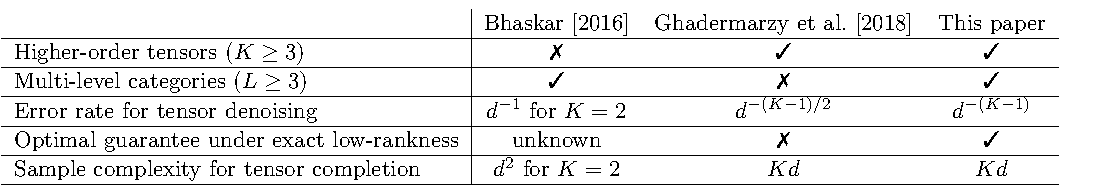
\includegraphics[width=16cm]{compare.pdf}}
\vspace{-.4cm}
\caption{Comparison of various low-rank estimation methods based on categorical observations. For an order-$K$ dimensional-$(d,\ldots,d)$ ordinal tensor with $L$-level observations, we report the error bound in the recovered signal (for tensor denoising) and required sample complexity (for tensor completion) as functions of tensor dimensions. {\color{red}(font in the table seems odd...)}}~\label{tab:compare}
\end{table*}

\section{Preliminaries}
Let $\tY\in\mathbb{R}^{d_1\times \cdots \times d_K}$ denote an order-$K$ $(d_1,\ldots,d_K)$-dimensional tensor. We use $y_\omega$ to denote the tensor entry indexed by $\omega$, where $\omega\in[d_1]\times\cdots\times[d_K]$.  The Frobenius norm of $\tY$ is defined as $\FnormSize{}{\tY}=\sum_\omega y^2_\omega$ and the infinity norm of $\tY$ is defined as $\mnormSize{}{\tY}=\max_{\omega}|y_\omega|$. We use $\tY_{(k)}$ to denote the unfolded matrix of size $d_k$-by-$\prod_{i\neq k}d_k$, obtained by reshaping the tensor along the mode-$k$. The Tucker rank of $\tY$ is defined as a length-$K$ vector $\mr = (r_1,\ldots,r_K)$, where $r_k$ is the rank of matrix $\tY_{(k)}$ for all $k \in[K]$. We say that an event $A$ occurs ``with very high probability'' if $\mathbb{P}(A)$ tends to 1 faster than any polynomial of tensor dimension $d_{\min}=\min\{d_1,\ldots,d_K\}$ as $d_{\min}\to\infty$.

We use lower-case letters (e.g., $a$, $b$, $c$) for scalars/vectors, upper-case boldface letters (e.g., $\mA$, $\mB$, $\mC$) for matrices, and calligraphy letters (e.g., $\tA$, $\tB$, $\tC$) for tensors of order three or greater. For ease of notation, we allow the basic arithmetic operators (e.g., $\leq, +, -$) to be applied to pairs of vectors in an element-wise manner. We use the shorthand $[n]$ to denote the $n$-set $\{1,\ldots,n\}$ for $n \in N_{+}$.

\section{Model formulation and motivation}
\subsection{Observation model}
Let $\tY$ denote an order-$K$ $(d_1,\ldots,d_K)$-dimensional tensor. Suppose the entries of $\tY$ are ordinal-valued, and the observation space consists of $L$ ordered categories, denoted by $[L]:=\{1,\ldots,L\}$. We propose a cumulative link model for the ordinal tensor $\tY=\entry{y_\omega}\in[L]^{d_1\times \cdots\times d_K}$. Specifically, assume the entries $y_\omega$ are (conditionally) independently distributed with cumulative probabilities:
\begin{equation}\label{eq:model}
\mathbb{P}(y_\omega\leq \ell)=f(\theta_\omega+b_\ell),\ \text{for all}\ \ell\in[L-1],
\end{equation}
where $\Theta=\entry{\theta_\omega}\in\mathbb{R}^{d_1\times \cdots \times d_K}$ is a continuous-valued parameter tensor satisfying certain low-dimensional structure (to be specified later), $\mb=(b_1,\ldots,b_{L-1})$ is a set of unknown scalars satisfying $b_1<\cdots <b_{L-1}$, and $f(\cdot):\mathbb{R}\mapsto[0,1]$ is a known, strictly increasing function. We refer to $\mb$ as the cut-off points and $f$ the link function. 

The formulation~\eqref{eq:model} imposes an additive model to the transformed probability of cumulative categories, rather than that of each single category. This modeling choice is to respect the ordering structure among the categories. For example, if we choose the inverse link $f^{-1}(x)=\log {x\over 1-x}$ to be the log odds, then the model~\eqref{eq:model} assumes linear spacing between the proportional odds:
\begin{equation}\label{eq:logodd}
\log {\mathbb{P}(y_{\omega}\leq \ell) \over \mathbb{P}(y_\omega >  \ell) } - \log {\mathbb{P}(y_{\omega}\leq {\ell-1}) \over \mathbb{P}(y_\omega >  {\ell-1}) } = b_\ell-b_{\ell-1},
\end{equation}
for all tensor entries $y_\omega$. When there are only two categories in the observation space (e.g. binary tensors), the cumulative model~\eqref{eq:model} is equivalent to the usual multinomial link model. In general, however, when the number of categories $L\geq 3$, the proportional odds assumption~\eqref{eq:logodd} is more parsimonious, in that, the ordered categories can be envisaged as contiguous intervals on the continuous scale, where the points of division are exactly $b_1<\cdots <b_{L-1}$. This interpretation will be made more explicit in the next section. 

\subsection{Latent-variable interpretation.} 

We show that the ordinal tensor model~\eqref{eq:model} is equivalent to an $L$-level quantization model on $\tY=\entry{y_\omega}$:
\begin{align}\label{eq:quantization}
y_\omega&=
\begin{cases}
1,& \text{if $y^*_\omega\in(-\infty, b_1]$},\\
2,& \text{if $y^*_\omega\in(b_1, b_2]$},\\
\vdots  &\vdots\\
L,& \text{if $y^*_\omega\in(b_{L-1}, \infty)$},\\
\end{cases}
\end{align}
for all $\omega\in[d_1]\times \cdots \times [d_k]$. Here, $\tY^*=\entry{y^*_{i_1,\ldots,i_K}}$ is a latent continuous-valued tensor following an additive noise model:
\begin{align}\label{eq:latent}
\KeepStyleUnderBrace{\tY^*}_{\text{latent continuous-valued tensor}}=\KeepStyleUnderBrace{\Theta}_{\text{signal tensor}}+\KeepStyleUnderBrace{\tE}_{\text{i.i.d.\ noise}},
\end{align}
where $\tE=\entry{\varepsilon_\omega}\in\mathbb{R}^{d_1\times \cdots \times d_K}$ is a noise tensor with i.i.d.\ entries following distribution $\tF(\varepsilon)$. From the viewpoint of~\eqref{eq:latent}, the parameter tensor $\Theta$ can be interpreted as the latent signal tensor prior to contamination and quantization. 

The equivalence between the latent-variable model~\eqref{eq:quantization} and the cumulative link model~\eqref{eq:model} is established if the link $f$ behaves like a cumulative distribution function of noise $\varepsilon$, i.e., $f(\theta)=\mathbb{P}(\varepsilon\geq -\theta)$. We describe several common choices of link $f$, or equivalently, the distribution of $\tE$. 

\begin{example}[Logistic model] The logistic model is characterized by~\eqref{eq:model} with $f(\theta)=(1+e^{-\theta/\sigma})^{-1}$, where $\sigma>0$ is the scale parameter. Equivalently, the noise $\varepsilon_\omega$ in~\eqref{eq:quantization} follows i.i.d.\ logistic distribution with scale parameter $\sigma$. 
\end{example}
\begin{example}[Probit model] The probit model is characterized by~\eqref{eq:model} with
$f(\theta)=\mathbb{P}(z\leq \theta/\sigma)$, where $z\sim N(0,1)$. Equivalently, the noise $\varepsilon_\omega$ in~\eqref{eq:quantization} follows i.i.d.\ $N(0,\sigma^2)$.
\end{example}
\begin{example}[Laplace model] The Laplacian model is characterized by~\eqref{eq:model} with
\[
f(\theta)=\begin{cases}
{1\over 2}e^{\theta\over \sigma}, & \text{if $\theta<0$},\\
1-{1\over 2}e^{-{\theta\over \sigma}}, & \text{if $\theta\geq 0$},
\end{cases}
\]
where $\sigma>0$ is the scale parameter. Equivalently, the noise $\varepsilon_\omega$ in~\eqref{eq:quantization} follows i.i.d.\ Laplace distribution with scale parameter $\sigma$. 
\end{example}
Other link functions are also possible, such as Cauchy function, inverse log-log, etc~\cite{mccullagh1980regression}. All the models share the property that the ordered categories can be thought of as contiguous interval on some continuous scale. We should point out that, although the latent-variable interpretation is incisive, our estimation procedure does not require the existence of $\tY^*$. Therefore, our model~\eqref{eq:model} is general and still valid in the absence of quantization process. More generally, we make the following assumptions to the link function $f$. 

\begin{assumption}\label{ass:link}
The link function is assumed to satisfy:
\vspace{-.4cm}
\begin{enumerate}
\item $f(\theta)$ is strictly increasing, strictly log-concave, and twice-differentiable in $\theta\in\mathbb{R}/\{0\}$.
\vspace{-.2cm}
\item $f'(\theta)$ is unimodal, and symmetric with respect to $\theta=0$. 
\end{enumerate}
\end{assumption}

\subsection{Problem 1: Tensor denoising.}~\label{sec:denoising}
The first question we aim to address is tensor denoising: 

(P1) Given the quantization process induced by $f$ and the cut-off points $\mb$, how accurate can we recover the latent signal tensor $\Theta$ from the ordinal observation $\tY$? 

Clearly, the problem (P1) cannot be solved uniformly for all possible $\Theta$. We focus on a class of ``low-rank'' and ``flat'' signal tensors, which is a plausible assumption in practical applications~\cite{zhou2013tensor,bhaskar20151}. Specifically, we consider the parameter space:
\begin{equation}\label{eq:space}
\small \tP=\left\{\Theta\in\mathbb{R}^{d_1\times \cdots \times d_K} \colon \text{rank}(\Theta)\leq \mr,\ \mnormSize{}{\Theta}\leq \alpha\right\}.
\end{equation}
where $\mr=(r_1,\ldots,r_K)$ denotes the Tucker rank of $\Theta$. 

The candidate tensor of our interest satisfies two constraints. The first is that $\Theta$ is a low-rank tensor, with $r_k=O(1)$ for all $k\in[K]$. The Tucker low-rankness is popularly used in tensor data analysis, and is shown to provide a reasonable tradeoff between model complexity and model flexibility. Note that, unlike matrices, there are various notations of tensor low-rankness, such as CP representation~\cite{hitchcock1927expression} and train representation~\cite{oseledets2011tensor}. Some notation of low-rankness may lead to mathematically ill-defined optimization; for example, the set of low-rank CP tensors is not necessarily compact~\cite{de2008tensor}. We choose Tucker representation for parsimony and easier interpretation. 

The second constraint is that the entries of $\Theta$ are uniformly bounded in magnitude by a constant $\alpha \in \mathbb{R}_{+}$. In view of~\eqref{eq:latent}, we refer to $\alpha$ as the signal level. The entry-wise bound assumption is a technical condition that ensures the well-posedness for the problems we considered. In the context of denoising with ordinal observations, the entry-wise bound helps avoid the degeneracy in probability estimation. 

\subsection{Problem 2: Tensor completion}
Motivated by applications in collaborative filtering and recommendation system, we also also consider a more general setup when only a subset of tensor entries $y_\omega$ are observed. Let $\Omega\subset[d_1]\times \cdots\times[d_K]$ denote the set of observed indices. The second question we aim to address is stated as follows:

(P2) Given an incomplete set of ordinal observation $\{y_{\omega}\}_{\omega\in\Omega}$ based on the model~\eqref{eq:model}, how many sampled entries do we need to consistently estimate $\Theta$? 

The answer to (P2) depends on the choice of $\Omega$. We propose a general model on $\Omega$ that allows both uniform and non-uniform sampling. Specifically, let $\Pi=\{\pi_{i_1,\ldots,i_K}\}$ denote a predefine probability distribution over the index set such that $\sum_{\omega\in[d_1]\times \cdots \times [d_K]} \pi_\omega =1$. We assume that each index in $\Omega$ are drawn with replacement using distribution $\Pi$. This model relaxes the the commonly-used uniform sampling and is arguably a better fit in practical applications. 

We consider the same parameter space~\eqref{eq:space} for the completion problem. In addition to the reasons mentioned in Section~\ref{sec:denoising}, the entrywise bound assumption also serves as the incoherence condition here. In classical matrix completion, the incoherence is often imposed on the singular vectors. This assumption was relaxed by considering ``flat'' matrices with bounded magnitude~\cite{negahban2011estimation,cai2013max,bhaskar20151}. We adopt the same assumption for higher-order tensors. 

\section{Rank-constrained M-estimator}
We present a general treatment to both problems mentioned above. With a little abuse of notation, we use $\Omega$ to denote either the full index set $\Omega=[d_1]\times \cdots \times [d_K]$ (for the tensor denoising) or a random subset induced from the sampling distribution $\Pi$ (for the tensor completion). Define $b_0=-\infty$, $b_L=\infty$, $f(-\infty)=0$ and $f(\infty)=1$. The log-likelihood associated with the observed entries is
\begin{align}\label{eq:objective}
\logl(\Theta, \mb)&=\sum_{\omega\in\Omega}\sum_{\ell\in[L]} \Big\{\mathds{1}_{\{y_\omega=\ell\}} \log \big[f(\theta_\omega+b_\ell)- \notag \\
&\quad \quad \quad \quad \quad \quad \quad  f(\theta_\omega+b_{\ell-1})\big]\Big\}.
\end{align}
We propose a rank-constrained maximum likelihood estimator (M-estimator) for $\Theta$:
\begin{align}\label{eq:estimator}
\hat \Theta&=\argmax_{\Theta\in \tP}\logl(\Theta, \mb),\ \text{where}\notag \\
\tP&=\left\{\Theta\in\mathbb{R}^{d_1\times \cdots \times d_K} \colon \text{rank}(\Theta)\leq \mr,\ \mnormSize{}{\Theta}\leq \alpha\right\}.
 \end{align}
 In practice, the cut-off points $\mb$ are unknown and should be jointly estimated with $\Theta$. For technical convenience, we assume that, in this section, the cut-off points $\mb$ are known, or otherwise have been consistently estimated {\color{red}(??)}. The adaptation of unknown $\mb$ will be addressed in Section~\ref{sec:algorithm}. Similar treatment applies to the hyper-parameter $\mr$. 

We define a few key quantities that will be used in our theory. Let $g_\ell=f(\theta+b_\ell)-f(\theta+b_{\ell-1})$ for all $\ell\in[L]$, and
\begin{align}\label{eq:regular}
A_\alpha &= \min_{\ell\in[L], |\theta|\leq \alpha} g_\ell(\theta),\quad  U_\alpha=\max_{\ell\in[L], |\theta|\leq \alpha } {\dot{g}_\ell(\theta)\over g_\ell(\theta)},\\
 L_\alpha &= \min_{\ell\in[L], |\theta|\leq \alpha }\left[{\dot{g}_\ell^2 (\theta)\over g_\ell^2(\theta)} -{\ddot{g}_\ell(\theta)\over g_\ell(\theta)}\right],
\end{align}
where $\dot{g}(\theta)=dg(\theta)/d\theta$, and $\alpha$ is the entrywise bound of $\Theta$. In view of equation~\eqref{eq:latent}, these quantities characterize the geometry (such as flatness and convexity) of the latent noise distribution. Under the Assumption~\ref{ass:link}, all these quantities are strictly positive and independent of tensor dimensions. 


\subsection{Estimation error for tensor denoising}
For the tensor denosing problem, we assume the full set of tensor entries are observed. In such a case, we assess the estimation accuracy using the mean squared error (MSE):
\[
\text{MSE}(\hat \Theta, \trueT)={1\over \prod_k d_k}\FnormSize{}{\Theta-\trueT}^2.
\]
The next theorem establishes the upper bound for the proposed $\hat \Theta$ in~\eqref{eq:estimator}. 

\begin{thm}[Statistical convergence] \label{thm:rate}
Consider an ordinal tensor $\tY\in[L]^{d_1\times\dots\times d_K}$ generated from model~\eqref{eq:model}, with the link function $f$ and the true coefficient tensor $\trueT\in\tP$. Define $r_{\max}=\max_k r_k$. Then, with very high probability, the estimator in~\eqref{eq:estimator} satisfies
\begin{equation}\label{eq:rate}
\text{MSE}(\hat \Theta, \trueT) \leq \min\left( 4\alpha^2,\ {c_2  U^2_\alpha r_{\max}^{K-1}  \over  L^2_\alpha } {\sum_kd_k\over  \prod_k d_k} \right),
\end{equation}
where $c_1, c_2>0$ are two constants that depend only on $K$. 
\end{thm}
Theorem~\ref{thm:rate} provides the statistical converge for the estimator~\eqref{eq:estimator}. Its proof is given in the Supplements. In fact, the proof of this theorem shows that the same statistical rate holds not only for the global optimizer of~\eqref{eq:estimator}, but also for any local optimizer $\check \Theta$ in the level set $\{\check\Theta\in\tP: \logl(\check\Theta)\geq \logl(\trueT)\}$. This suggests that the local optimality itself is not necessarily a severe concern in our context, as long as the objective value at the estimator is large enough. In Section~\ref{sec:simulation}, we will perform empirical studies to assess the algorithmic stability and its impact to statistical efficiency. 

A similar conclusion can be obtained for the prediction error, measured in Kullback-Leibler (KL) divergence, between the two categorical distributions. 
\begin{cor}[Prediction error]~\label{cor:prediction}
Assume the same set-up as in Theorem~\ref{thm:rate}. Let $\mathbb{P}_{\tY}$ and $\hat{\mathbb{P}}_{\tY}$ denote the distributions generating the $L$-level ordinal tensor $\tY$, given the true parameter $\Theta$ and its estimator $\hat \Theta$, respectively. Assume $L\geq 2$. Then, with very high probability, 
\begin{equation}\label{eq:KLrate}
\text{KL}(\mathbb{P}_{\tY} || \hat{\mathbb{P}}_{\tY}) \leq  {c_2 U^2_\alpha r_{\max}^{K-1}  \over L^2_\alpha } {(4L-6)\dot{f}^2(0)  \over A_\alpha} {\sum_kd_k\over  \prod_k d_k},
\end{equation}
where $c_1, c_2>0$ are the same constants as in Theorem~\ref{thm:rate}.  
\end{cor}
To gain insight into these bounds, we consider a special setting where the dimensions are the same in all modes, i.e., $d_1=\cdots=d_K=d$. In such a case, our bound \eqref{eq:rate} reduces to
\begin{equation*}\label{eq:ours}
\text{MSE}(\hat \Theta, \trueT) \asymp d^{-(K-1)}, \quad \text{as}\ d\to \infty.
\end{equation*}
Hence, the estimator achieves consistency with polynomial convergence rate. Comparing to max norm based estimator $\tilde{\Theta}$ proposed by~\citet{ghadermarzy2018learning}, $\text{MSE}(\tilde{\Theta}, \trueT) \asymp  d^{-(K-1)/2}$, we see that our bound has a faster convergence rate. We believe the improvement comes from utilizing the exact low-rank structure of $\Theta$, whereas an scale-sensitive surrogate rank measure was employed in~\citet{ghadermarzy2018learning}. 

Our bound also generalizes the previous results on ordinal matrices. The convergence rate for rank-constrained matrix denoising was $O(1/\sqrt{d})$~\citep{bhaskar2016probabilistic}, which fits into our special case when $K=2$. Furthermore, our results~\eqref{eq:rate} and~\eqref{eq:KLrate} reveal that the convergence becomes favorably as the order of tensor data increases. 
Intuitively, for tensor data analysis, the sample size is the number of tensor entries, $\prod_k d_k$, and the number of free parameters is roughly on the order of $\sum_{k}d_k$, assuming $r_{\max}=O(1)$. A higher tensor order implies higher effective sample size per parameter, and thus exhibits a faster convergence rate in high dimensions. 


We next establish the statistical optimality of our estimator $\hat \Theta$. The result is based on the information theory, and therefore applies to all estimators in $\tP$, including but not limited to $\hat \Theta$ in~\eqref{eq:estimator}. We show that this lower bound matches the upper bound in~\eqref{eq:rate} as a function of tensor dimensions. 


\begin{thm}[Minimax lower bound]\label{thm:minimax} 
Assume the same set-up as in Theorem~\ref{thm:rate}, and $d_{\max}=\max_k d_k \geq 8$. Let $\inf_{\hat \Theta}$ denote the infimum over all estimators $\hat \Theta\in\tP$ based on the ordinal tensor observation $\tY\in[L]^{d_1\times \cdots \times d_K}$. Then, under the model~\eqref{eq:model},
\begin{align}\label{eq:lower}
\inf_{\hat \Theta }\sup_{\trueT\in\tP} \mathbb{P}\Big\{& \text{MSE}(\hat \Theta, \trueT) \\
& \geq {1\over 256} \min\left( \alpha^2, \ { Cr_{\max}d_{\max} \over \prod_k d_k} \right) \Big\} \geq {1\over 8},
\end{align}
where $C=C(\alpha, L, f,\mb)>0$ is a constant independent of tensor dimensions and the rank. 
\end{thm}


\subsection{Sample complexity for tensor completion}

Now we consider the problem of tensor completion, when only a subset of entries $\Omega$ are observed. We consider a general sampling procedure induced by $\Pi$. The recovery accuracy is assessed by the weighted squared deviation:
\begin{align}\label{eq:weighted}
\PiFnormSize{}{\Theta-\hat \Theta}^2&\stackrel{\text{def}}{=}
{1\over |\Omega|}\mathbb{E}_{\Omega\sim \Pi}\FnormSize{}{\Theta-\hat \Theta}^2\notag \\
&=\sum_{\omega\in[d_1]\times \cdots \times [d_K]} \pi_{\omega}(\Theta_{\omega}-\hat \Theta_{\omega})^2.
\end{align}

Note that the recovery error depends on the distribution $\Pi$. In particular, the entries with higher sampling probabilities are equipped with better accuracy guarantee, compared to the ones with lower sampling probabilities. 

\begin{rmk} If we assume each tensor entry is sampled with some positive probability, i.e., there exits a constant $\mu> 0$ such that 
\[
\pi_\omega\geq {1\over \mu \prod_k d_k},\quad \text{for all}\quad \omega\in[d_1]\times\cdots \times [d_K],
\]
then the error measure in~\eqref{eq:weighted} provides an upper bound for MSE:
\[
\PiFnormSize{}{\Theta-\hat \Theta}^2 \geq {\FnormSize{}{\Theta-\hat \Theta}^2\over \mu \prod_kd_k}={1\over \mu}\text{MSE}(\hat \Theta, \trueT).
\]
The equality is attained in the case of uniform sampling for which $\mu=1$. 
\end{rmk}


\begin{thm}~\label{thm:completion}
Assume the same set-up as in Theorem~\ref{thm:rate}. Suppose that we observe a subset of tensor entries $\{y_\omega\}_{\omega\in\Omega}$, where $\Omega$ is chosen at random with replacement according to a probability distribution $\Pi$. Let $\hat \Theta$ be the solution to~\eqref{eq:estimator}, and assume $r_{\max}=O(1)$. Then, with very high probability over the sampled set $\Omega$ ({\color{red} not over $\tY$?}), 
\[
\PiFnormSize{}{\Theta-\hat \Theta}^2 \to 0,\quad \text{ as }\quad {|\Omega|\over \sum_k d_k} \ \to \infty. 
\]
\end{thm}
Theorem~\ref{thm:completion} shows that our estimator achieves consistency when sample size is greater than $O(\sum_k d_k)$. {\color{red} add remarks comparing with prior work, and with the degree of freedom.}

\section{Numerical Implementation}\label{sec:algorithm}
\subsection{Alternating optimization}


\begin{algorithm}[tb]
        \caption{Ordinal tensor decomposition }\label{alg}
        \begin{algorithmic}[]
            \STATE{\bfseries Input:}  \text{ Ordinal tensor }
            $\mathcal{Y}\in [L]^{d_1\times\cdots\times d_K}
            $,\\ \hspace{.43in} Rank $\mr\in \mathbb{N}_+^{K}$,\\
            \hspace{.43in} Entry-wise bound $\alpha\in \mathbb{R_+}$.
            \STATE{\bfseries Output:} $(\hat\Theta,\hat{\mb}) =  \argmax_{(\Theta,\mb)\in \mathcal{D}\times\mathcal{B}}  \mathcal{L}_{\mathcal{Y},\Omega}(\Theta,\mb).$
            \STATE Initialize  Core tensor $\mathcal{C}^{(0)}$,\\
            \hspace{.5in} Factor matrices $ \{\mM_1^{(0)},\cdots,\mM_K^{(0)}\}$,\\
            \hspace{.5in} Cut-off points $\mb^{(0)}$.
            \FOR{$t = 1,2,\cdots,$}
            \FOR{$k = 1,2,\cdots,K$}
            \STATE{Update $\mM_k$ while fixing other blocks.}
            \STATE $\mM_k^{(t+1)}\gets\argmax_{\mM_k\in\mathbb{R}^{d_k\times r_K}}\mathcal{L}_{\mathcal{Y},\Omega}(\mM_k)$
            \newline
             s.t. $\mnormSize{}{\Theta^{(t+1)}}\leq \alpha$, where $\Theta^{(t+1)}$ is the parameter tensor based on the current block estimates. 
            \ENDFOR
            \STATE {Update $\mathcal{C}$ while fixing other blocks: $\mathcal{C}^{(t+1)} \gets \argmax_{\mathcal{C}\in \mathbb{R}^{r_1\times\cdots\times r_K}}\mathcal{L}_{\mathcal{Y},\Omega}(\mathcal{C})$, s.t. $\mnormSize{}{\Theta^{(t+1)}}\leq \alpha$. 
               \STATE {Update $\Theta$ based on the current block estimates: $\Theta^{(t+1)} \gets \mathcal{C}^{(t+1)}\times_1\mM_1^{(t+1)}\cdots\times_K\mM_K^{(t+1)}$. 
            \STATE {Update $\mb$ while fixing $\Theta^{(t+1)}$: $\mb^{(t+1)} \gets \argmax_{\mb\in \mathbb{R}^{L-1}}\mathcal{L}_{\mathcal{Y},\Omega}\big(\Theta^{(t+1)},\mb\big)$
            \ENDFOR
            \STATE \textbf{return}
            $\Theta,\mb$
        \end{algorithmic}
    \end{algorithm}

In this section, we describe the algorithm to seek the optimizer of~\eqref{eq:objective}. The objective function $\logl(\Theta)$ is concave in $\Theta$ whenever $\tP$ is log-concave~\cite{mccullagh1980regression}. However, the feasible set $\tP$ is not a convex set, which makes the optimization~\eqref{eq:objective} a non-convex problem. One approach to handle this problem is utilizing the Tucker decomposition and converting optimization into a block-wise convex problem. Let us denote the low Tucker-rank tensor as
\begin{equation}\label{eq:Tucker}
\Theta=\tC\times_1\mM_1\times_1 \cdots \times_K \mM_K,
\end{equation}
where $\tC\in\mathbb{R}^{r_1\times \cdots \times r_K}$ is a core tensor and $\mM_k\in\mathbb{R}^{d_k\times r_k}$ are factor matrices with orthogonal columns. From~\eqref{eq:objective} and \eqref{eq:Tucker}, we have $K+2$ blocks of variables in the objective function, one for the cut-points vector $\mb$, one for the core tensor $\tC$, and $K$ for the factor matrices $\mM_k$'s. We can change the optimization problem to simple convex problem if any $N+1$ out of the $N+2$ blocks being fixed. Therefore, we can update one block at a time while other blocks being fixed, and alternate the optimization via iteration. The Algorithm 1 gives the full description.

{\color{red} (highlight that $\mb$ and $\Theta$ are jointly estimated...)}


\subsection{Tuning parameter selection}\label{sec:BIC}
Algorithm~1 takes the rank $\mr$ as an input. In practice, the rank $\mr$ is hardly known and needs to be estimated from the data. We suggest to use Bayesian information criterion (BIC) and choose the rank that minimizes BIC; i.e.
\begin{align}\label{eq:BIC}
\hat \mr&=\argmin_{\mr\in\mathbb{N}^K_{+}} \text{BIC}(\mr)\\
&=\argmin_{\mr\in\mathbb{N}^K_{+}}\left[-2\tL_{\tY}(\hat \Theta(\mr))+p_e(\mr)\log \left(\prod_k d_k\right) \right],
\end{align}
where $\hat \Theta(\mr)$ is the estimator given the rank $\mr$, and $p_e(\mr)\stackrel{\text{def}}{=}\sum_k (d_k-r_k)r_k+\prod_k r_k$ is the effective number of parameters in the model. We select the rank $\hat \mr$ that minimizes BIC through a grid search. Our choice of BIC aims to balance between the goodness-of-fit for the data and the degree of freedom in the population model. We test its empirical performance in Section~\ref{sec:simulation}. 


\section{Experiments}
In this section, we evaluate the empirical performance of our rank-constrained estimation. We consider ordinal tensors with various number of categories, and compare the recovery accuracy with other tensor-based methods. Unless otherwise stated, we generate ordinal-valued tensor under the latent-variable model~\eqref{eq:latent} with i.i.d.\ $N(0,\sigma^2)$ noise. The signal tensor is simulated based on~\eqref{eq:Tucker}, with core tensor generated from i.i.d. N(0,1), and the factor matrices uniformly from orthogonal ensembles. The cut-off points are generated i.i.d.from $N(0,1)$. In each simulation study, we report the summary statistics across $n_{\text{sim}}$ = 30 replications.

\subsection{Finite-sample performance}\label{sec:simulation}

\subsection{Comparison with alternative methods}


\section{Real data application}
In this section, we apply our ordinal tensor decomposition method to two real-world datasets of ordinal tensors. In the first application, we use our model to analyze an ordinal tensor consisting of structural connectivity patterns among 68 brain regions for 136 individuals from Human Connectome Project (HCP) (Geddes 2016). In the second application, we perform tensor completion from the data with missing values. The data tensor records the ratings from scale 1 to 5 of 42 users to 139 songs on 26 contexts (Baltrunas et al. 2011).

\subsection{Human Connection Project (HCP)}
The human connectome project (HCP) is a 68 � 68 � 136 tensor where the first two modes have 68 indices representing brain regions and the last mode has 136 indices meaning individuals. All the individual images were preprocessed following a standard pipeline (Zhang et al. 2018), and the brain was parcellated to 68 regions of interest following the Desikan atlas (Desikan et al. 2006). The tensor entries consist of $\{1, 2, 3\}$, the strength of fiber connections between 68 brain regions for each of the 136 individuals. First, we apply our ordinal tensor decomposition method with a logistic link function to the HCP data and identify similar brain nodes based on latent parameters. The BIC result suggests $\mr = (23, 23, 8)$ with $\logl(\hat \Theta,\hat \mb) = - 216645.8$.

Also, we compare our ordinal tensor decomposition method with a logistic link function with the classical continuous Tucker decomposition method. We use 5 folded cross validation method for the comparison. Specifically, we randomly split the tensor entries into 5 similar sized pieces and alternatively use each piece of entries as a test data using other 80\% entries as a training data. The entries in the test data are encoded as missing and then predicted based on the tensor decomposition from the training data. We set the rank of the tensor as $\mr = (23,23,8)$ which minimizes BIC value. Table 1 shows RMSE, MAE and error (false prediction rate), averaged over 5 test set results. We can check that our ordinal tensor decomposition model outperforms the classic continuous decomposition in all criteria.

%\begin{table}[H]
%\resizebox{\linewidth}{!}{%
%\begin{tabular}{c|ccc|c}
%\hline
%\multirow{2}{*}{Critera}&\multicolumn{3}{c|}{Our method}&Continuous method\\
%& $\hat y^{(\text{Mean})}_\omega$ & $\hat y^{(\text{Median})}_\omega$ & $\hat y^{(\text{Mode})}_\omega$ &~\cite{filipovic2015tucker}\\
%\hline
%MSE& &  & 0.1504&0.1604\\
%MAD&  &  &0.1504&0.1600\\
%MCR& &&0.1502&0.1598\\
%\hline
%\end{tabular}
%}
%\caption{Comparison of tensor denoising on HCP dataset.}
%\end{table}



\subsection{InCarMusic recommendation system}
InCarMusic is a mobile application that offers music recommendation to passengers of cars based on contexts (Baltrunas et al. 2011). Our goal is to perform the tensor completion to the $42\times 139\times 26$ ordinal tensor and thereby we can offer context-specific music recommendation to users. The tensor entries consist of ordinal observations on the scale 1 to 5, the ratings of 42 users to 139 songs on 26 contexts and are encoded as NA for missing values. The number of missing values is 148,904 and the number of available values is 2,884.
We suggest three estimators $\hat y_\omega$ based on $(\hat \theta_\omega,\hat \mb)$:
\begin{itemize}
\item (Mean) $\hat y^{(\text{Mean})}_\omega=\sum_\ell \ell g_\ell(\hat \theta_\omega,\hat \mb) $;
\item (Median) $\hat y^{(\text{Median})}_\omega=\min\{\ell\in[L]\colon f_\ell(\hat \theta_\omega,\hat \mb)\geq 0.5\}$;
\item (Mode) $\hat y^{(\text{Mode})}_\omega=\argmax_\ell g_\ell(\hat \theta_\omega,\hat \mb) $
\end{itemize}
Note that, under the ordinal tensor model~\eqref{eq:model}, the estimator $\hat y^{(\text{Mean})}_\omega$ (uniformally?) minimizes $\mathbb{E}(y_\omega-\hat y_\omega)^2$, and the estimator $\hat y^{(\text{Median})}_\omega$ minimizes $\mathbb{E}|y_\omega-\hat y_\omega|$ (?). In contrast, these three estimators degenerate to a single estimator under the continuous-valued tensor decomposition model. We assess the accuracy using three metrics: Mean squared error (MSE), Mean absolute deviation (MAD), and Misclassification rate (MCR).  

Results are averaged from 5 fold cross validation. {\color{red} add s.e. to the above table.} 

\begin{table}[H]
\resizebox{\linewidth}{!}{%
\begin{tabular}{c|ccc|c}
\hline
\multirow{2}{*}{Critera}&\multicolumn{3}{c|}{Our method}&Continuous method\\
& $\hat y^{(\text{Mean})}_\omega$ & $\hat y^{(\text{Median})}_\omega$ & $\hat y^{(\text{Mode})}_\omega$ &~\cite{filipovic2015tucker}\\
\hline
MSE& \color{red}2.01&2.14 & 3.64&8.18\\
MAD& 1.23  &  {\color{red}1.13}&1.26&2.36\\
MCR& 0.80&0.75&{\color{red}0.54}&0.96\\
\hline
\end{tabular}
}
\caption{Comparison of tensor completion performance on InCarMusic dataset.}
\end{table}

We also attempted to run matrix ordinal mehod~\citep{bhaskar2016probabilistic} to the InCarMusic dataset. Unfortunately, the $\mb$ cannot be estimated from their method. 

\bibliography{tensor_wang}
\bibliographystyle{icml2020}


\end{document}


% This document was modified from the file originally made available by
% Pat Langley and Andrea Danyluk for ICML-2K. This version was created
% by Iain Murray in 2018, and modified by Alexandre Bouchard in
% 2019 and 2020. Previous contributors include Dan Roy, Lise Getoor and Tobias
% Scheffer, which was slightly modified from the 2010 version by
% Thorsten Joachims & Johannes Fuernkranz, slightly modified from the
% 2009 version by Kiri Wagstaff and Sam Roweis's 2008 version, which is
% slightly modified from Prasad Tadepalli's 2007 version which is a
% lightly changed version of the previous year's version by Andrew
% Moore, which was in turn edited from those of Kristian Kersting and
% Codrina Lauth. Alex Smola contributed to the algorithmic style files.
